
\documentclass{beamer}

\usepackage{algpseudocode, color, colortbl}

\usepackage{hyperref}
\hypersetup{
    colorlinks=true,
    urlcolor=blue,
}

\usetheme{Montpellier}
\usecolortheme{rose}

% page numbers, from
% https://tex.stackexchange.com/questions/137022/how-to-insert-page-number-in-beamer-navigation-symbols
\expandafter\def\expandafter\insertshorttitle\expandafter{%
  \insertshorttitle\hfill%
  \insertframenumber\,/\,\inserttotalframenumber}

\definecolor{Gray}{gray}{0.8}
\newcolumntype{g}{>{\columncolor{Gray}}c}

\newcommand{\stanza}{ \\~\ }

\title{09. Linear Programming Generalizations}
\subtitle{CPSC 535 $\sim$ Spring 2019}
\author{Kevin A. Wortman}
\institute{ 
\includegraphics[height=2cm]{csuf-logo-cmyk} }
\date{April 15, 2019 \stanza

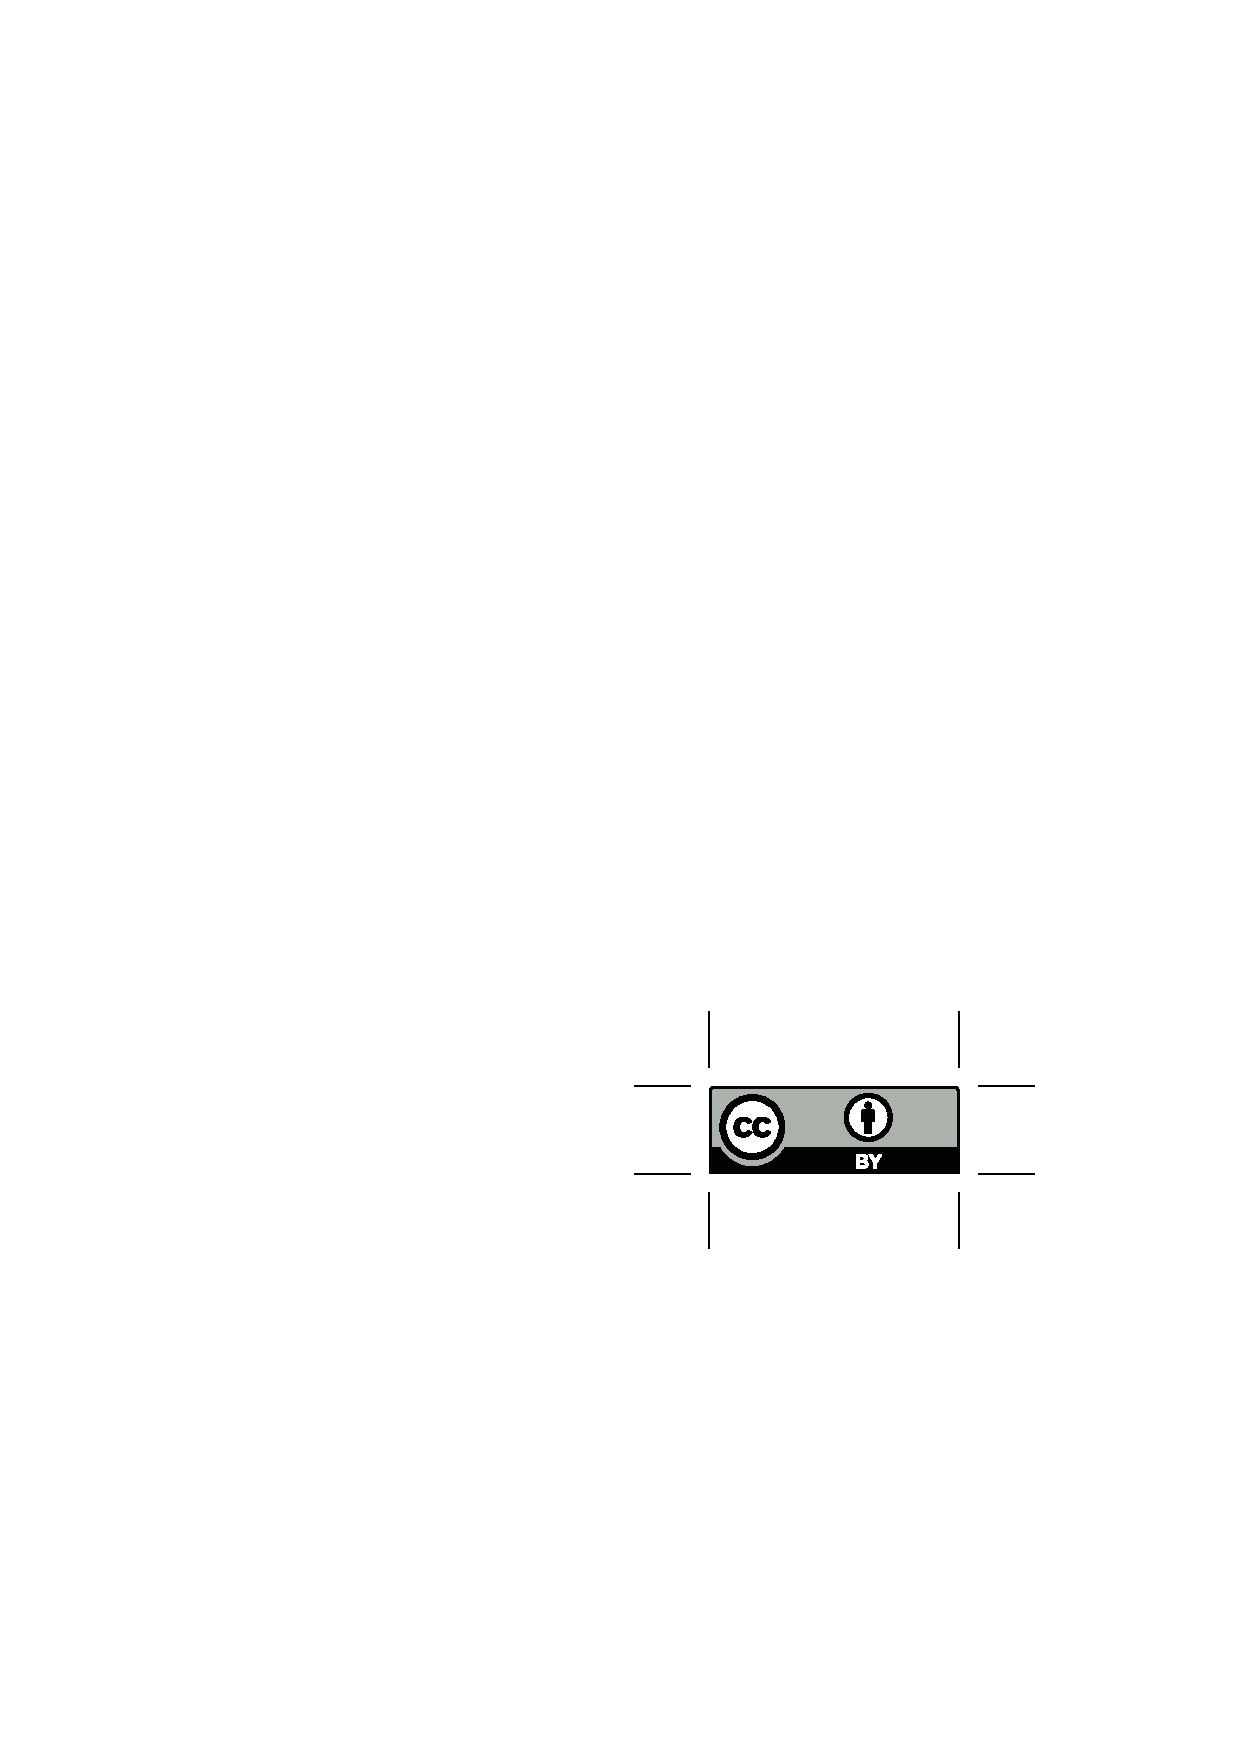
\includegraphics[height=14pt]{by} \\

{\tiny
This work is licensed under a
\href{http://creativecommons.org/licenses/by/4.0/}{Creative Commons Attribution 4.0 International License}.
}}

\begin{document}

\begin{frame}
  \titlepage
\end{frame}

\begin{frame} \frametitle{Big Idea from Algorithm Design: Duality}
  \textbf{Duality:} When a mathematical object fits two different human models,
    we can view that object in two ways, (1) \emph{primal} and (2) \emph{dual.} \stanza

  $\implies$ one algorithm could solve two different problems, (1) primal-based
    and (2) dual-based. \stanza

  Consequently
  \begin{itemize}
    \item one algorithm actually solves two problems
    \item two perspectives on the same problem could inspire problem-solving
    \item reasoning about dual could be easier than primal
  \end{itemize}
\end{frame}

\begin{frame} \frametitle{Big Idea from Algorithm Design: Parameterized Tractibility}
Idea: Sometimes we can overcome efficiency barriers by designing an algorithm that
is fast in terms of a parameter that scales up (e.g. $n$), but slow in terms of a
parameter that doesn't in practice (e.g. $W$).

Recall
\begin{itemize}
\item decision sorting must take $\Omega(n \log n)$ time (barrier)
\item radix sort takes $\Theta(nW)$ time; faster when $W \in O(1)$ (faster in practice,
  if not technically faster in theory)
\end{itemize}

Linear Programming (LP)
\begin{itemize}
  \item fast (polynomial) on practical inputs
  \item seems to take worst-case exponential time in theory
  \item fast pseudopolynomial time i.e. $O((d+n)^{1.5} d W)$
  \item dimension (\# variables) is $O(1)$, fast linear time $O(n)$
\end{itemize}
\end{frame}

\begin{frame} \frametitle{Example: lines and points}
Primal: set of lines $\{ (m, b) : m, b \in \mathbb{R} \}$ \\
Dual: set of 2D points $\{ (x, y) : x, y \in \mathbb{R} \}$ \stanza

Observe: math, and computer, can't distinguish between lines and points!
A function that does something to a set of lines, also does something to a set of points. \stanza

\emph{parallel line search} \\
\textbf{input:} a set $L = \{ (m, b) : m, b \in \mathbb{R} \}$ of lines \\
\textbf{output:} two lines $(m_1, b_1), (m_2, b_2)$ that are parallel, or NIL
if no such lines exist \stanza

Question: what is the dual of this problem? \\
\emph{Hint:} replace ``line'' $\rightarrow$ ``point,'' $m \rightarrow x, b \rightarrow y$
\end{frame}

\begin{frame} \frametitle{Duality in the Simplex Algorithm}
\textbf{Idea:} view solving an LP in terms of \emph{two} related programs
\begin{enumerate}
  \item primal LP: original input; goal is to maximize objective function
  \item dual LP: minimize ``slack'' between left-hand-side of inequalities and
    right-hand-side
\end{enumerate}

Recall: optimal solutions may always be found on simplex vertices
\begin{enumerate}
  \item in the primal: objective function ``pushes'' us toward a vertex
  \item in the dual: minimizing slack ``pulls'' us toward an inequality (line/hyperplane)
\end{enumerate}
\end{frame}

\begin{frame} \frametitle{Standard Form to Slack Form}
A standard-form inequality looks like
\[ 7 x_1 + 3 x_2 \leq 4 \]

Equivalently we may introduce variable $s$ representing the \emph{slack}
or difference between the left-hand-side and right-hand-side.
\[ 7 x_1 + 3 x_2 + s = 4 \]
\[ s \geq 0 \]
(note that $\leq$ turned into $=$)

\end{frame}

\begin{frame} \frametitle{Simplex Algorithm (High-Level)}
\begin{enumerate}
  \item Find an initial \emph{feasible solution} inside the simplex of feasible solutions.
    (Usually trivial.)
  \item \textbf{repeat}:
    \begin{enumerate}
      \item Find a variable with positive slack in all inequalities.
      \item If no such variable exists, \textbf{stop}.
      \item Eliminate slack; increase var's with positive coefficients, or decrease
        var's with negative coefficients, until some inequality has zero slack.
      \item \emph{Pivot:} This variable/inequality in the primal is maxxed out and
        cannot be optimized again; exchange it for an inequality/variable in the dual.
      \end{enumerate}
\end{enumerate}
\end{frame}

\begin{frame} \frametitle{Simplex Algorithm Analysis}
With $d$ variables and $n$ inequalities, the body of the loop is $\Theta(dn).$ \stanza

\# iterations = number of times one variable gets maxxed out before reaching optimal solution
(not a function of $d, n$) \stanza

In practice (e.g. last week's exercise), \# iterations is $\sim d, n$ so simplex algorithm
takes polynomial time. \stanza

Surprise: $\exists$ carefully-crafted LP for which simplex algorithm takes exponential
time (e.g. \emph{Klee-Minty cube}) \stanza

Worst-case analysis approach is unsatisfying here; can be shown that average runtime
is polynomial when averaging over random LPs.
\end{frame}

\begin{frame} \frametitle{Pseudopolynomial Time Algorithms}
After the simplex algorithm was analyzed formally, researchers designed algorithms with provable pseudopolynomial. For word size $W, d$ variables, and $n$ inequalities,
\begin{itemize}
  \item Khachiyan's \emph{ellipsoid algorithm} takes $O(d^4 W)$ time.
  \item \emph{Vaidya's algorithm} takes $O((d+n)^{1.5} d W)$ time.
  \item (there are others)
\end{itemize}

Mostly of theoretical interest; simplex algorithm remains faster on practical LPs. \stanza

Open research questions
\begin{enumerate}
  \item Is there an LP algorithm that runs in pseudopolynomial time \emph{and} is faster than simplex in practice?
  \item Is LP in $P$? $\Leftrightarrow$ Is there an LP algorithm that runs in strongly polynomial time (function of only $d, n$, not $W$)?
\end{enumerate}
\end{frame}

\begin{frame} \frametitle{Integer Linear Programming}
\textbf{Integer Linear Programming (ILP)}: same form as LP, but every variable must
be an integer, not real number. \stanza

maximize $\mathbf{c}^T \mathbf{x}$ \\
subject to $A \mathbf{x} \leq \mathbf{b}$ and $\mathbf{x} \geq \mathbf{0}$ \\
\underline{and $\mathbf{x} \in \mathbb{Z}^d$} \stanza

\textbf{Mixed Integer Linear Programming (MILP)}: \emph{some} variables must be
integers, others may be any real (integer or not). \stanza

Both are $NP$-complete; exponential-time only (assuming $P \ne NP$).
\end{frame}

\begin{frame} \frametitle{Applications of ILP, MILP}
Can use an integer variable to choose between discrete alternatives. \stanza

Can introduce indicator variables to decide to use/not use something; e.g.
whether an edge is part of a minimum spanning tree.
\begin{itemize}
  \item Create variable $x \in \mathbb{Z}$
  \item $0 \leq x$
  \item $x \leq 1$
\end{itemize}
\end{frame}

\begin{frame} \frametitle{Example: Latin Squares}
\textbf{input}: $n \times n$ grid with some elements filled with $1, \ldots, n$ \\
\textbf{output}: each element filled with $1, \ldots, n$ such that each value
appears exactly once per row and once per column; or NIL if this is impossible \stanza
\begin{center}
\begin{tabular}{|c|c|c|c|} \hline
   1 &   &    \\ \hline
     & 2 & 1  \\ \hline
   2 &   &    \\ \hline
\end{tabular}
$\Longrightarrow$
\begin{tabular}{|c|c|c|c|} \hline
   1 & 3 & 2  \\ \hline
   3 & 2 & 1  \\ \hline
   2 & 1 & 3  \\ \hline
\end{tabular}
\end{center}
\end{frame}

\begin{frame} \frametitle{Latin Squares formulated as ILP}
For each row $i$, column $j$, value $v$, each in $1, \ldots, n$, introduce
indicator variable
\[ g_{i, j, k} = 1 \Leftrightarrow \text{assign value } k \text{ to row $i$, col. $j$} \]

\begin{tabular}{ll}
  $0 \leq g_{i, j, k} \leq 1$ & $\forall i, j, k$ (each indicator is 0 or 1) \\
  $g_{i, j, k} = x$ & for all pos'n $i, j$ pre-filled to $x$ \\
  $\sum_{j} g_{i, j, k} = 1$ & $\forall i, k$ (each value appears once per row) \\
  $\sum_{i} g_{i, j, k} = 1$ & $\forall j, k$ (each value appears once per column) \\
  $g_{i, j, k} \in \mathbb{Z}$ & $\forall i, j, k$ (indicators are integers) \\
\end{tabular}

\end{frame}

\begin{frame} \frametitle{Low-Dimensional LP}
Megiddo: algorithm with runtime
\[ O(c^d n) \]
for $c>1$;
\begin{itemize}
  \item exponential in $d$, still counts as exponential time
  \item \textbf{but}, when $d \in O(1)$, this simplifies to
  \[ O(c^d n) = O((1) n) = O(n) \]
  \item $\implies$ \textbf{linear time} when number of variables $d$ is a small
    constant
\end{itemize}
\end{frame}

\begin{frame} \frametitle{Generalizations of Low-Dimensional LP}
More general objective functions still admit $O(c^d n)$-time algorithms
\begin{enumerate}
  \item \emph{quadratic} programming e.g. maximize $f(x_1, \ldots, x_d) = $ (polynomial of order 2)
  \item \emph{cubic} programming e.g. maximize $f(x_1, \ldots, x_d) = $ (polynomial of order 3)
  \item \emph{convex} programming e.g. maximize $f,$ a \emph{convex} function
  \item \emph{quasiconvex} programming, e.g. maximize $f,$ a \emph{quasiconvex} function
\end{enumerate}

Inequalities are still linear in these frameworks.\\
Applications include geometric problems (points, lines, circles, etc.).
\end{frame}

\end{document}
